\documentclass[12pt]{article}
	
\usepackage[margin=1in, left=0.6in, right=0.6in]{geometry}
\usepackage{fancyhdr}	% header
\usepackage{hyperref} % links

%\usepackage[edges]{forest}
%\usepackage{tikz-qtree}

\usepackage{amsmath,amsthm,amssymb}	%math stuff
\usepackage{graphicx} \graphicspath{ {./images/} }
%\usepackage{array}
\usepackage{setspace} % increase line spacing
\usepackage{tabularx} % long tables
\usepackage{enumitem} % labelling itmes
% \usepackage{relsize} 

\pagestyle{fancy}
\fancyhead[LO,L]{CSCB63 A1}
\fancyhead[CO,C]{Stephen Guo}
\fancyhead[RO,R]{1006313231}
\fancyfoot[LO,L]{}
\fancyfoot[CO,C]{\thepage}
\fancyfoot[RO,R]{}

\newcommand{\N}{\mathbb{N}}
\newcommand{\R}{\mathbb{R}}
\newcommand{\Rplus}{\mathbb{R}^{+}}
\newcommand{\bigbracket}[1]{\big(#1\big)}
\newcommand{\Bigbracket}[1]{\Big(#1\Big)}
\newcommand{\floorSurround}[1]{\left\lfloor#1\right\rfloor}
\newcommand{\ceilingSurround}[1]{\left\lceil#1\right\rceil}
%\newcommand{\code}[1]{\verb | #1 |}
\renewcommand{\qed}{\hfill$\blacksquare$}

\begin{document} %\setstretch{1.2}
%----------------------------------------------------------------------------------
%                              Table of Contents
%----------------------------------------------------------------------------------
\begin{center}
	\hypertarget{toc}{\LARGE \noindent \underline{\textbf{Table of Contents}}}\\
\end{center}
\noindent \textbf{Question 1:}
\vspace{1mm}
\hrule
\vspace{1mm}
\noindent\hyperlink{1.1}{(a)}\\
\hyperlink         {1.2}{(b)}\\

\noindent \hyperlink{2}{\textbf{Question 2:}}
\vspace{1mm}
\hrule
\vspace{1mm} \leavevmode \\

\noindent \hyperlink{3}{\textbf{Question 3:}}
\vspace{1mm}
\hrule
\vspace{1mm} \leavevmode \\

\noindent \hyperlink{4}{\textbf{Question 4:}}
\vspace{1mm}
\hrule
\vspace{1mm} \leavevmode \\

% \noindent \hyperlink{5}{\textbf{Question 5:}}
% \vspace{1mm}
% \hrule
% \vspace{1mm} \leavevmode \\
\newpage
%{\setstretch{1.5}$\begin{array}{r@{}>{\displaystyle}l}  \end{array}$}
%----------------------------------------------------------------------------------
%                                   Questions
%----------------------------------------------------------------------------------
%----------------------------------------------------------------------------------
% !                                    1
%----------------------------------------------------------------------------------
{\LARGE \noindent \underline{\textbf{Question 1.}}}\\

\noindent \hyperlink{toc}{\hypertarget{1.1}{(a)}} % ! %%%%%%%%%%%   (a)    %%%%%%
{\setstretch{1.5}$$\begin{array}{r@{}>{\displaystyle}l}
			A(n)   & {}=n^2 A(n-1) \hspace*{20mm} \\
			A(n-1) & {}= (n-1)^2 A(n-2)           \\
			A(n-2) & {}= (n-2)^2 A(n-3)           \\
			       & {}\hspace*{2.4mm} \vdots     \\
			A(2)   & {}= (2)^2A(1)                \\
			A(1)   & {}= 1
		\end{array}$$}
\\
\text{So by \textbf{Repeated Back Substitution,} we have: }
{\setstretch{1.5}$$\begin{array}{r@{}>{\displaystyle}l}
			A(n) & {}= n^2 (n-1)^2 (n-2)^2 \cdots (2)^2 (1)^2   \\
			     & {}= \bigbracket{n(n-1)(n-2) \cdots (2)(1)}^2 \\
			     & {}= (n!)^2                                   \\
		\end{array}$$}
$$\therefore A(n) \in \Theta\big((n!)^2\big)$$
\\\\
\newpage
\noindent \hyperlink{toc}{\hypertarget{1.2}{(b)}}\\ % ! %%%%%%%%%%%   (b)    %%%%%%
$$
	C(n) = \left\{
	\begin{aligned}
		8C\floorSurround{\frac{n}{2}} + 2n^3 + 4n \qquad & \hspace*{3mm}\text{ if } n > 0 \\
		6 \qquad                                         & \hspace*{3mm}\text{ if } n = 0 \\
	\end{aligned}
	\right.
$$
\\\\
We can calculate $C(1)$ by plugging it in.
	{\setstretch{1.5}$$\begin{array}{r@{}>{\displaystyle}l}
				C(1) & {} = 8C\floorSurround{\frac{1}{2}} + 2(1)^3 + 4(1) \hspace*{10mm} \\
				     & {} = 8C(0) + 2 + 4                                                    \\
				     & {} = 8(6) + 6                                                     \\
				     & {} = 54                                                           \\
      \end{array}$$}
Now we can rewrite $C(n)$ to...
$$
	C(n) = \left\{
	\begin{aligned}
		8C\floorSurround{\frac{n}{2}} + 2n^3 + 4n \qquad & \hspace*{3mm}\text{ if } n > 1 \\
		54 \qquad                                         & \hspace*{3mm}\text{ if } n = 1 \\
	\end{aligned}
	\right.
$$
\\\\
We can see that this sastisfies the \textbf{Generalized Master Theorem}, where
\\\\
% \begin{tabularx}{\textwidth}{
% 		>{\centering\arraybackslash}X
% 		>{\centering\arraybackslash}X
% 		>{\centering\arraybackslash}X
% 		>{\centering\arraybackslash}X
% 		>{\centering\arraybackslash}X
% 	}
% 	$a = 8 $ &
% 	$b=2 $   &
% 	$c=2$    &
% 	$d=6$    &
% 	$f(n) = 2n^3 + 4n$
% \end{tabularx}
\begin{tabular*}{\textwidth}{c @{\extracolsep{\fill}} cccc}
	$a = 8 $ &
	$b=2 $   &
	$c=3$    &
	$d=54$    &
	$f(n) = 2n^3 + 4n$
\end{tabular*}
\\\\
So we know that $f(n) \in \Theta(n^3)$, and $\log_2 8 = 3$\\
$\Longrightarrow \log_b a = c$
\\\\
By part (b) of \textbf{Generalized Master Theorem}, we have
\[
	{\setstretch{1.5}\begin{array}{r@{}>{\displaystyle}l}
				T(n) & {}= \Theta(n^{\log_b a}  \log_bn) \\
				     & {}= \Theta(n^3  \log_2n)          \\
			\end{array}}
\]
\newpage
%----------------------------------------------------------------------------------
% !                                    2
%----------------------------------------------------------------------------------
\noindent\hyperlink{toc}{\hypertarget{2}{\LARGE \noindent \underline{\textbf{Problem 2.}}}}
\\\\
Suppose... \\
\begin{tabular*}{\textwidth}{c @{\extracolsep{\fill}} ccc}
	$f(n) \in \mathcal{O}\bigbracket{g(n)}$ &
	$f(n) \geq 1 $   &
	$\log \bigbracket{g(n)} \geq 1$    &
	$\forall n \in \N$
\end{tabular*}\ \\
%$f(n) \in \mathcal{O}\bigbracket{g(n)}$
\begin{itemize}[leftmargin=14mm]
	\item[\textbf{WTS}:]  $\log \bigbracket{f(n)} \in \mathcal{O}\Bigbracket{\log\bigbracket{g(n)}}$ \textbf{\qquad OR}\\
	      $\exists c' \in \Rplus,\ \exists n_0' \in \N,\ \forall n > n_0'\ \Longrightarrow\ \log \bigbracket{f(n)} \leq c' \cdot \log \bigbracket{g(n)}$
	      \qquad \textbf{($\bigstar$)}\\
\end{itemize}
Since $f(n) \in \mathcal{O}\bigbracket{g(n)}$ we have...\\
$\exists c \in \Rplus,\ \exists n_0 \in \N,\ \forall n > n_0\ \Longrightarrow\ f(n) \leq c \cdot g(n)$\\
{\setstretch{1.5}$$\begin{array}{r@{}>{\displaystyle}ll}
		f(n)                   & {} \leq  c \cdot g(n)                                                         & [\text{by given}]                                   \\
		\log \bigbracket{f(n)} & {}\leq \log \bigbracket{c\cdot g(n)}                                          & [\text{logging both sides since both sides }\geq 1] \\
		                       & {}\leq \log(c) + \log \bigbracket{g(n)}                                       & [\text{by log laws}]                                \\
		                       & {}\leq  \log(c) \log \bigbracket{g(n)}+ \log \bigbracket{g(n)} \hspace*{10mm} & [\text{since }\log \bigbracket{g(n)} \geq 1]        \\
		                       & {}\leq \bigbracket{\log(c) +1}\log \bigbracket{g(n)}                          & [\text{by factoring}]                               \\
	\end{array}$$}
\\
So choose: \hspace*{10mm} \\ $c' = \log(c) +1 \hspace*{10mm} n_0' = n_0$\\[2ex]
% \begin{tabularx}{\textwidth}{
%   >{\centering\arraybackslash}X
%   >{\centering\arraybackslash}X
% }
% $c' = \log(c) +1$ &
% $n_0' = n_0$
% \end{tabularx}
Then the predicate \textbf{($\bigstar$)} holds \qed
\newpage
%----------------------------------------------------------------------------------
% !                                    3
%----------------------------------------------------------------------------------
\noindent\hyperlink{toc}{\hypertarget{3}{\LARGE \noindent \underline{\textbf{Problem 3.}}}}
\begin{flushleft} \hyphenpenalty=10000 \exhyphenpenalty=10000
\textbf{Implementation:}\\
for \verb|RECENT|, I would use an \verb|AVL Tree| and a \verb|Doubly Linked List|.\\
I would also keep track of \verb|size|, and the \verb|head| and \verb|tail| of the \verb|Doubly Linked List|.
\\\ \\
In the \verb|AVL Tree|, the nodes would have an extra parameter:\\ 
\verb|target|: a pointer to its node in the \verb|Doubly Linked| \verb|List|.
\\\ \\
For every \verb|ACCESS(x)|, it would insert \verb|x| into both the \verb|AVL Tree| and the \verb|Doubly Linked List|.\\
If \verb|x| is already in the \verb|AVL Tree|, then use \verb|target| to delete that node in the \verb|Doubly Linked List|.
Then re-insert it back into the head of the \verb|Doubly Linked List| by using \verb|head|. 
\\\ \\
If \verb|size > m|, then delete both \verb|tail|, and its corresponding node in the \verb|AVL Tree|. Then continue to insert \verb|x|.
\\\ \\\
\\
\textbf{Justification:}\\
This data structure uses $\mathcal{O}(m \log n)$ space since we have 2 data structures of size \verb|m|.
This means that we will only have about \verb|2m| nodes to store, which according to \href{https://piazza.com/class/kju7e2uwa8p3sf?cid=55}{this piazza post},
takes about $2(m \log n) = \mathcal{O}(m \log n)$ space
\\\ \\
This data structure takes worst case $\mathcal{O}(\log m)$ time complexity. This is because for every \verb|ACCESS(x)|,
we need to search the \verb|AVL Tree| which takes $\mathcal{O}(\log m)$ time. It could also delete and insert in the \verb|Doubly Linked List| after searching,
which would take $\mathcal{O}(1)$ since we keep a pointer to \verb|size|, \verb|head|, and \verb|tail|.
Lastly, we would also need to delete from both the \verb|AVL Tree| and the \verb|Doubly Linked List| if \verb|size| gets too large,
which would take $\mathcal{O}(\log m)$ and $\mathcal{O}(1)$ time respectively.\\
Overall, the worst case time complexity is $\mathcal{O}(\log m)$. \end{flushleft}
% for \verb|RECENT|, I would use a \verb|queue| with an extra variable: \verb|size|.
% \\\\
% For every \verb|ACCESS(x)|, it would check if \verb|1 <= x <= n|.\\
% If it's \verb|true|, \verb|size++|, and we add \verb|x| to the \verb|queue|. \\
% If \verb|size > m|, then we would remove the last element in the \verb|queue|.
% \\\\
% We have worst time complexity $O(\log m)$ since adding or removing anything from the \verb|queue| would only take $O(1)$ time, 
% which is less than $O(\log m)$.
% \\\\
% This data structure would only take up $O(m \log n)$ space (\href{https://piazza.com/class/kju7e2uwa8p3sf?cid=55}{according to this piazza post})
% since\\ every number takes $\log(n)$ space, and we can only have max $m$ elemnts in the queue.\\
% So our upper-bound of our data structure for space complexity is $m \times \log(n)$ 
\newpage
%----------------------------------------------------------------------------------
% !                                    4
%----------------------------------------------------------------------------------
\noindent\hyperlink{toc}{\hypertarget{4}{\LARGE \noindent \underline{\textbf{Problem 4.}}}}
\begin{center}
  \def \imageWidth {5.7in}
	Tree after inserting 5, 4, 6, 9, 12, 16, 14, 2, 3\\
  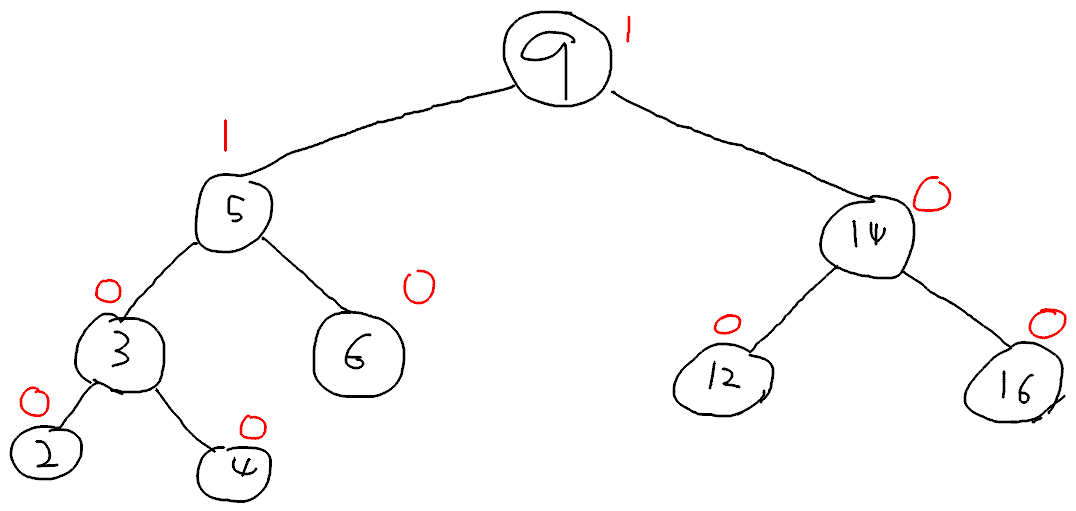
\includegraphics[width=\imageWidth]{CSCB63_A1_4a.png}\\\ \\
  
	Tree after inserting 1, 20, 19, 18, 17\\
  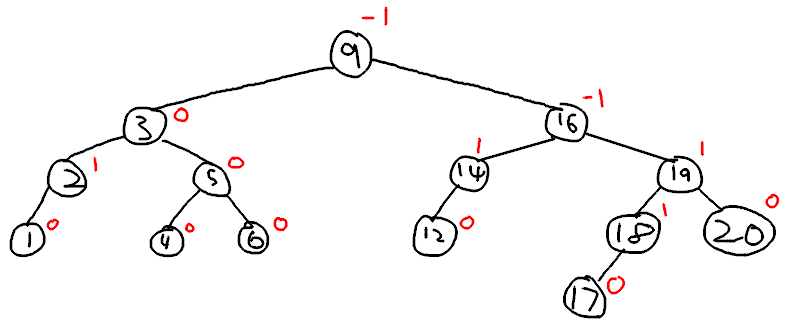
\includegraphics[width=\imageWidth]{CSCB63_A1_4b.png}\\\ \\

  Tree after deleting 1, 2, 3, 4, 5, 12, 6\\
  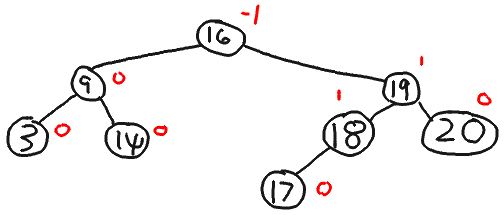
\includegraphics[width=\imageWidth]{CSCB63_A1_4c.png}
\end{center}
\newpage
%----------------------------------------------------------------------------------
% !                                    5
%----------------------------------------------------------------------------------
% \noindent\hyperlink{toc}{\hypertarget{5}{\LARGE \noindent \underline{\textbf{Problem 5.}}}}
% \\\\


% \newpage

\end{document}